\section{JPA: Object Relational Mapping}

The technique of bridging the gap between the object model and the relational model is known as object-relational mapping. 
\begin{definition}[\textit{Impedance mismatch}]
    The challenge of mapping one model to the other lies in the concepts in one model for which there is no logical equivalent in the other, referred to as impedance mismatch.
\end{definition}
The automatic transformation of a model into another in managed by an element called mediator. 
The principal distinctions between the object-oriented model and the relational one are as follows:
\begin{table}[H]
    \centering
    \begin{tabular}{cc}
    \hline
    \textbf{Object-oriented model}     & \textbf{Relational model}   \\ \hline
    Objects, classes                   & Tables, rows                \\
    Attributes, properties             & Columns                     \\
    Identity (physical memory address) & Primary key                 \\
    Reference to other entity          & Foreign key                 \\
    Inheritance/Polymorphism           & Not supported               \\
    Methods                            & Stored procedures, triggers \\
    Code is portable                   & Not necessarily portable    \\ \hline
    \end{tabular}
\end{table}
The Java Persistence API addresses the gap between object-oriented domain models and relational database systems by utilizing Plain Old Java Objects, providing a persistence model for object-relational mapping.

\paragraph*{Features}
Key features of the Java Persistence API include:
\begin{itemize}
    \item \textit{POJO Persistence}: objects being persisted need not possess any special characteristics; any existing non-final object with a default constructor can be persisted.
    \item \textit{Non-intrusiveness}: the persistence API exists as a separate layer from the persistent objects.
    \item \textit{Object queries}: a powerful query framework offers the ability to query across entities and their relationships without having to use concrete foreign keys or database columns.
\end{itemize}

\begin{definition}[\textit{Entity}]
    The entity is a class (Java bean) representing a collection of persistent objects mapped onto a relational table. 
\end{definition}
\begin{definition}[\textit{Persistence unit}]
    The persistence unit is the set of all classes that are persistently mapped to one database (analogous to the notion of db schema). 
\end{definition}
\begin{definition}[\textit{Persistence context}]
    The persistence context is the set of all managed objects of the entities defined in the persistence unit (analogous to the notion of db instance). 
\end{definition}
\begin{definition}[\textit{Managed entity}]
    The managed entity is an entity part of a persistence context for which the changes of the state are tracked. 
\end{definition}
\begin{definition}[\textit{Entity manager}]
    The entity manager is the interface for interacting with a persistence context. 
\end{definition}
\begin{definition}[\textit{Client}]    
    The client is a component that can interact with a persistence context, indirectly through an entity manager.
\end{definition}
Entities are accessed through the entity manager interface of the Java Persistence API.
\begin{figure}[H]
    \centering
    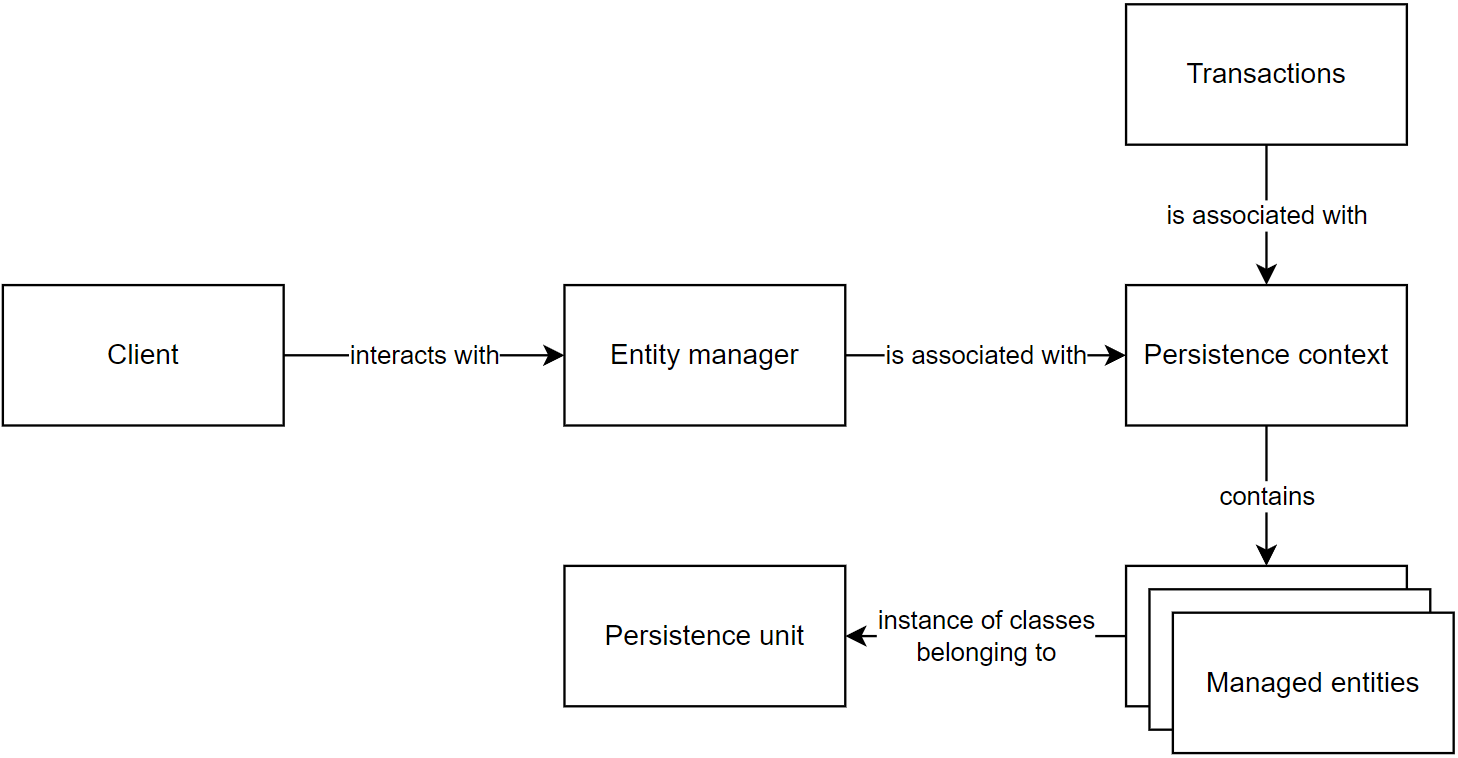
\includegraphics[width=0.75\linewidth]{images/jpa.png}
    \caption{Structure of the Java Persistence API}
\end{figure}

\paragraph*{Interfaces}
The entity manager exposes all the operations needed to synchronize the managed entities in the persistence context to the database to:
\begin{itemize}
    \item Persist an entity instance in the database: \texttt{public void persist(Object entity)}.
    \item Find an entity instance by its primary key. 
        The method's signature to accomplish this is: \texttt{public <T> T find(Class<T> entityClass, Object primaryKey)}.
    \item Remove an entity instance from the database: \texttt{public void remove(Object entity)}.
    \item Reset the entity instance from the database: \texttt{public void refresh(Object entity)}.
    \item Write the state of entities to the database immediately: \texttt{public void flush()}.
\end{itemize}

\paragraph*{Entities}
An entity is a Java Bean associated with a tuple in a database. 
The persistent counterpart of an entity has a lifespan longer than that of the application.
The entity class must be associated with the database table it represents. 
An entity can enter a managed state, where all modifications to the object's state are tracked and automatically synchronized to the database.
Entities have properties such as identification (primary key), nesting, relationship, referential integrity (foreign key), and inheritance. 
Entities must meet certain requirements:
\begin{itemize}
    \item Must have a public or protected constructor with no arguments.
    \item Must not be final.
    \item No method or persistent instance variables may be final.
    \item The Serializable interface must be implemented if you pass the entity by value.
\end{itemize}
In the database, objects and tuples have an identity (primary key), so an entity assumes the identity of the persistent data it is associated with.
The primary key can be either simple or composite. 
To identify a primary key, we use the \texttt{@Id} annotation, and for composite keys, we use \texttt{@EmbeddedId} and \texttt{@IdClass} annotations.

\paragraph*{Uniqueness of data}
At times, applications may prefer not to handle the explicit management of data value uniqueness. 
In such scenarios, the persistence provider has the capability to automatically create an identifier for each entity instance of a specified type. 
This functionality, known as identifier generation, is defined by the \texttt{@GeneratedValue} annotation. 
There are four available ID generation strategies that applications can opt for:
\begin{enumerate}
    \item \texttt{Auto}. 
    \item \texttt{Table}: identifiers are generated based on a generator table.
    \item \texttt{Sequence}: the identifiers are generated using sequences. 
    \item \texttt{Identity}: the identifiers are generated using primary keys identity columns. 
\end{enumerate}
\begin{example}
    An identifier can be generated as follows: 
    \begin{lstlisting}[style=Java]
@Entity
public class Mission implements Serializable {
@Id
@GeneratedValue(strategy = GenerationType.IDENTITY)
private int id;
private String city;
}
    \end{lstlisting}
\end{example}
Attributes can be qualified  with properties that guide the mapping between Plain Old Java Objects (POJO) and relational tables. 
These properties include: large objects, enumerated types, and temporal types. 

\paragraph*{Fetch policies}
The fetch policy can be either lazy (retrieve the item when needed) or eager (retrieve the item as soon as possible).
Lazy policy is primarily employed for large objects.
\begin{example}
    The qualifiers can be used as follows: 
    \begin{lstlisting}[style=Java]
@Entity
public class Mission implements Serializable {
@Id
@GeneratedValue(strategy = GenerationType.IDENTITY)
private int id;
@Temporal(TemporalType.DATE)
private Date date;
private MissionStatus status;
@Basic(fetch=FetchType.LAZY)
@LOB
private byte[] photo;
}
    \end{lstlisting}
\end{example}
Entities are ordinarily mapped to tables with corresponding names, and their fields are mapped to columns with identical names by default.
However, it is possible to alter this behavior using certain annotations.
In cases where an entity should not be persisted, it can be designated with the \texttt{@Transient} annotation.
\begin{example}
    The mapping can be redefined as follows: 
    \begin{lstlisting}[style=Java]
@Entity @Table(name="T_BOOKS")
public class Book {
@Column(name="BOOK_TITLE", nullable=false)
private String title;
private CoverType coverType;
private Date publicationDate;
@Transient
private BigDecimal discount;
}
    \end{lstlisting}
\end{example}

\subsection{Mapping}
In any object model, relationships exhibit four key characteristics:
\begin{itemize}
    \item \textit{Directionality}: each of the two entities involved may possess an attribute that facilitates access to the other entity.
        If two entities are mutually connected, it forms a bidirectional relationship; otherwise, it constitutes a unidirectional relationship.
        Multiple references are possible.
    \item \textit{Role}: each entity within the relationship plays a role in one direction of access. 
        Entities are categorized as source and target based on the relationship's direction.
    \item \textit{Cardinality}: this refers to the number of instances of entities on each side of the relationship.
        Four cardinality possibilities exist: 
        \begin{itemize}
            \item \textit{Many-to-one}: many source entities to one target entity.
            \item \textit{One-to-many}: one source entity to many target entities.
            \item \textit{One-to-one}: one source entity to one target entity.
            \item \textit{Many-to-many}: many source entities to many target entities.
        \end{itemize}
    \item \textit{Ownership}: in a relationship, one of the two entities is deemed the owner.
        In the database, relationships are implemented through a foreign key column (referred to as the join column in JPA) that points to the key of the referenced table. 
        The entity with a foreign key column is considered the owner of the relationship, and its side is termed the owning side.
\end{itemize}

\paragraph*{One-to-many relationship}
The bidirectional one-to-many relationship is established using the \texttt{mappedBy}, \texttt{@ManyToOne}, and \texttt{@OneToMany} annotations, where:
\begin{itemize}
    \item \texttt{@ManyToOne} annotation is applied to the entity participating with multiple instances, designating the entity containing this annotation as the owner of the relationship.
    \item \texttt{@JoinColumn} annotation is utilized to specify the foreign key column of the underlying table.
\end{itemize}
\begin{example}
    Here's the first part of the definition for a one-to-many bidirectional mapping:
    \begin{lstlisting}[style=Java]
@Entity
public class Employee {
@Id private int id;
@ManyToOne
@JoinColumn(name="dept_fk")
private Department dept;
}
    \end{lstlisting}
\end{example}
To achieve bidirectionality, the mapping direction for the one-to-many relationship must also be specified.
This is accomplished by including a \texttt{@OneToMany} annotation in the entity participating with one instance.
The \texttt{@OneToMany} annotation is placed on a collection data member and includes a \texttt{mappedBy} element to indicate the property implementing the inverse of the relationship.
\begin{example}
    Here's the second part of the definition for a one-to-many bidirectional mapping:
    \begin{lstlisting}[style=Java]
@Entity
public class Department {
@Id private int id;
@OneToMany(mappedBy="dept")
private Collection<Employee> employees;
}
    \end{lstlisting}
\end{example}
In cases where applications only require access to relationships along one direction, bidirectional mapping may not be necessary.

\paragraph*{Many-to-one relationship}
The many-to-one relationship is defined in the same way as the one-to-many, but the source and the target are switched in the definition. 

\paragraph*{One-to-one relationship}
To establish a one-to-one relationship in JPA, two alternative approaches can be chosen:
\begin{itemize}
    \item Map the relationship similarly to the bidirectional case and utilize only the one-to-many direction.
    \item Omit the mapping of the collection attribute in the entity participating with one instance, and instead, use a query to retrieve correlated instances, relying on the inverse (many-to-one) relationship direction mapping.
\end{itemize}
The distinction between \texttt{@joincolumn} and \texttt{mappedby} is as following: 
\begin{itemize}
    \item The \texttt{@joincolumn} annotation specifies the foreign key column implementing the relationship in the database. 
        This annotation is typically applied to the entity that owns the relationship and aids in generating SQL code for extracting correlated instances.
    \item The \texttt{mappedby} attribute indicates that this side is the inverse of the relationship, with the owner residing in the other related entity. 
        It is used to define bidirectional relationships. 
        In the absence of the mappedBy parameter, the default JPA mapping involves a bridge table.
\end{itemize}
In a one-to-one mapping, the owner can be either entity, depending on the database design. 
A one-to-one mapping is declared by annotating the owner entity with the \texttt{@OneToOne} annotation.
\begin{example}
    Here's the first part of the definition for a one-to-one mapping:
    \begin{lstlisting}[style=Java]
@Entity
public class Employee {
@Id private int id;
@OneToOne
private ParkingSpace parkingSpace;
}
    \end{lstlisting}
\end{example}
For bidirectional one-to-one mapping, the inverse side of the relationship must also be specified. 
In the non-owner entity, both the \texttt{@OneToOne} annotation and the \texttt{mappedBy} element are needed to guide JPA in placing the foreign key.
\begin{example}
    Here's the second part of the definition for a one-to-one mapping:
    \begin{lstlisting}[style=Java]
@Entity
public class ParkingSpace {
@Id private int id;
@OneToOne(mappedBy="parkingSpace")
private Employee employee;
}
    \end{lstlisting}
\end{example}

\paragraph*{Many-to-many relationship}
In a many-to-many mapping, there is no foreign key column, but instead, a join table is utilized. 
Consequently, either entity can be arbitrarily designated as the owner.
\begin{example}
    Here's the first part of the definition for a many-to-many mapping:
    \begin{lstlisting}[style=Java]
@Entity
public class Employee {
@Id private int id;
@ManyToMany
private Collection<Project> projects;
}
    \end{lstlisting}
\end{example}
For bidirectional many-to-many mapping, the inverse side of the relationship must also be specified. 
In the non-owner entity, both the \texttt{@ManyToMany} annotation and the \texttt{mappedBy} element are required.
\begin{example}
    Here's the second part of the definition for a many-to-many mapping:
    \begin{lstlisting}[style=Java]
@Entity
public class Project {
@Id private int id;
@ManyToMany(mappedBy="projects")
private Collection<Employee> employees;
}
    \end{lstlisting}
\end{example}
The logical model of a many-to-many relationship necessitates a bridge table (join table in JPA).
\begin{example}
    Here's an example specifying the non-default mapping of the entity to the bridge table via annotations:
    \begin{lstlisting}[style=Java]
@Entity
public class Employee {
@Id private long id;
private String name;
@ManyToMany
@JoinTable(name="EMP_PROJ",
        joinColumns=@JoinColumn(name="EMP_ID"),
        inverseJoinColumns=@JoinColumn(name="PROJ_ID"))
private Collection<Project> projects;
}
    \end{lstlisting}
\end{example}

\subsection{Relationship fetch mode}
When the fetch mode is unspecified, the default behavior is as follows:
\begin{itemize}
    \item Single-valued relationships are fetched eagerly.
    \item Collection-valued relationships are loaded lazily.
\end{itemize}
In the case of bidirectional relationships, the fetch mode may be lazy on one side but eager on the other. 
It's important to note that the recommended practice is to consider lazy loading as the most suitable mode for all relationships.
This is because if an entity has many single-valued relationships that are not all utilized by applications, eager loading may result in performance drawbacks.
\begin{example}
    Here's an example using the annotation to define lazy loading:
    \begin{lstlisting}[style=Java]
@Entity
public class Employee {
@Id private int id;
@OneToOne(fetch=FetchType.LAZY)
private ParkingSpace parkingSpace;
}
    \end{lstlisting}
\end{example}
It's essential to understand that the directive to lazily fetch an attribute serves as a hint to the persistence provider, which retains the flexibility to employ an eager loading policy if deemed necessary. 
However, the reverse is not true: the eager policy cannot be replaced with a lazy one by the provider.

\subsection{Cascading operations}
By default, every operation performed by the entity manager does not cascade to other entities that have a relationship with the entity being operated on.
However, in certain cases, it might be desirable to propagate changes to entities in a relationship with the modified one. 
This can be achieved by enabling manual cascading.
\begin{example}
    Here's an example illustrating the activation of manual cascading:
    \begin{lstlisting}[style=Java]
Employee emp = new Employee();
Address addr = new Address();
emp.setAddress(addr);
em.persist(addr);
em.persist(emp);
    \end{lstlisting}
    With manual cascading activated, when the entity manager adds the Employee instance to the persistence context, it navigates the address relationship, searching for a new Address entity to manage as well.
    The Address instance must be set on the Employee instance before invoking \texttt{persist()} on the employee object.  
    If an Address instance has been set on the Employee instance and not persisted explicitly or implicitly via cascading, an error occurs.
\end{example}
The \texttt{cascade} attribute is used to specify when operations should automatically cascade across relationships, accepting values such as: \texttt{persist}, \texttt{refresh}, \texttt{remove}, \texttt{merge}, and \texttt{detach}.
If all the previous operations are desired, the \texttt{all} operator can be used.
\begin{example}
    Activation of manual cascading of type persist: 
    \begin{lstlisting}[style=Java]
@Entity
public class Employee {
@ManyToOne(cascade=CascadeType.PERSIST)
Address address;
}
    \end{lstlisting}
\end{example}
It's important to note that cascade settings are unidirectional and must be set on both sides for bidirectional behavior.

\paragraph*{Cascade remove}
JPA also supports an additional remove cascading called \texttt{orphanRemoval}. 
This is utilized in \texttt{@OneToOne} and \texttt{@OneToMany} annotations for privately owned parent-child relationships where each child entity is associated only with one parent entity through just one relationship
This operation causes the child entity to be removed when the parent-child relationship is broken by removing the parent, setting to null the attribute holding the related entity, or in the one-to-many case, by removing the child entity from the parent's collection.
The distinction between the attribute \texttt{CascadeType.REMOVE} and the mode \texttt{orphanRemoval}  is that if the value of an entity is manually set to null, only \texttt{orphanRemoval} will automatically remove the linked entities from the database.